\title{Singularity Software\\Milestone 3}
\date{\today}

\documentclass[12pt]{article}
\usepackage[a4paper]{geometry}
\usepackage{makeidx}
\usepackage[acronym]{glossaries}
\usepackage{lscape}
\usepackage{amsmath}
\usepackage{graphicx}
\usepackage[final]{pdfpages}
% \usepackage{hyperref} % Makes links from ToC

\geometry{top=1.0in, bottom=1.0in, left=1.0in, right=1.0in} % Sets the margins

\setlength{\parindent}{0pt} % Fixes the paragraph spacing problem

% This is all for formatting and making the Table of Contents according to 
% spec. Don't play with it.
\makeatletter
\renewcommand\l@section[2]{%
  \ifnum \c@tocdepth >\z@
    \addpenalty\@secpenalty
    \addvspace{1.0em \@plus\p@}%
    \setlength\@tempdima{1.5em}%
    \begingroup
      \parindent \z@ \rightskip \@pnumwidth
      \parfillskip -\@pnumwidth
      \leavevmode \bfseries
      \advance\leftskip\@tempdima
      \hskip -\leftskip
      #1\nobreak\ 
      \leaders\hbox{$\m@th\mkern \@dotsep mu\hbox{.}\mkern \@dotsep mu$}
     \hfil \nobreak\hb@xt@\@pnumwidth{\hss #2}\par
    \endgroup
  \fi}
\makeatother

\makeindex

% Construct the glossary here
% Use the template below, then where the word appears (in the case below, computer), replace computer with \gls{computer}
\makeglossaries

\newglossaryentry{Sifteo Cubes}
{
  name={Sifteo Cubes},
  description={are small machines capable of loading programs and interacting with one another as well as responding to predefined movements}
}

\newglossaryentry{Object-Oriented Programming}
{
  name={Object-Oriented Programming},
  description={is a programming paradigm using objects to design applications}
}

\newglossaryentry{Windows}
{
  name={Windows},
  description={is a series of operating systems developed by Microsoft}
}

\newglossaryentry{Mac}
{
  name={Mac},
  description={is a series of lines of personal computers developed by Apple}
}

\newglossaryentry{Linux}
{
  name={Linux},
  description={is a Unix-based operating system based on free and open source software}
}

\newglossaryentry{cross-platform support}
{
  name={cross-platform support},
  description={is an attribute given to software implemented and operable on multiple computer platforms}
}

\newacronym{API}{API}{\glsadd{API}{Application Programming Interface}}

\newglossaryentry{APIg}
{
  name={Application Programming Interface},
  description={is an interface implemented by a software program that enables it to interact with other software}
}


\newglossaryentry{open source}
{
  name={open source},
  description={is an attribute given to software for which the source code is freely available}
}

\newacronym{IDE}{IDE}{\glsadd{IDE}{Integrated Development Environment}}

\newglossaryentry{IDEa}
{
  name={Integrated Development Environment},
  description={is software that provides a comprehensive work environment for computer programmers and software developers}
}


\newacronym{GUI}{GUI}{\glsadd{GUI}{Graphical User Interface}}

\newglossaryentry{GUIa}
{
  name={Graphical User Interface},
  description={is a visual way of allowing the user to interace with a computer program}
}

\newglossaryentry{version control}
{
  name={version control},
  description={is the management of documents and programs for a project over many versions in a well-organized manner}
}

\newglossaryentry{issue tracking system}
{
  name={issue tracking system},
  description={is a piece of software used to maintain a list of issues as generated during a project}
}

\renewcommand*\arraystretch{1.5}

\begin{document}
\vspace*{\fill}
        \begin{center}
                \LARGE{Singularity Software} \\
                \LARGE{\textit{Milestone 3}} \\
                \vspace{.15in}
                \large{\today} \\
                \vspace{4in}
                By signing below, I approve the contents of the following document. \\
                \begin{table}[h]
                        \begin{tabular}{p{2in} p{5.5in}}
%                \begin{align*}
                        & \\
                        Alex Mullans & \line(1,0){285} \\ & \\
                        Ruben Rodriguez & \line(1,0){285} \\ & \\
                        Ethan Veatch & \line(1,0){285} \\ & \\
                        Kurtis Zimmerman & \line(1,0){285}
                        \end{tabular}
                \end{table}
%                \end{align*}
        \end{center}
\vspace*{\fill}
\thispagestyle{empty}

\clearpage

\tableofcontents

\clearpage
        
\section{Executive Summary}
This document is the second in a series of milestone documents that will accompany the planning of the Siftables\index{Siftables} Emulator\index{emulator}. The Emulator project is a first of its kind application that will allow developers of Sifteo applications to test the features of the cubes in a virtual programming environment. Currently, the only way to test apps developed for the Sifteo Cubes platform is with the physical cubes; this project will eliminate that need and serve as a demo for the possibilities of the Sifteo platform.\\\\
This milestone elaborates the functional features of the the Siftables\index{Siftables} Emulator\index{emulator} project. It first gives a brief background of the project before moving on to elaborate features with use cases and declarative statements, where appropriate. It also maps all covered use cases to their relevant features. Finally, it presents mockups of the Emulator's design for consideration and to solicit client feedback.  Future milestones will present plans for change control, coding standardization, and testing. Finally, design and usability reports will make up the core of milestones near the end of the quarter as the software stabilizes.


\section{Introduction}
Developers of applications for the \gls{Sifteo Cubes}\index{Sifteo} currently must test programs they create for the platform on the Cubes themselves.  With a full release of the Cubes and corresponding \gls{API}\index{API}\glsadd{APIg} still pending, developers unable to join the Sifteo Early Access program are left without a software-based interface within which to productively develop Sifteo programs. As such, Singularity Software will provide, in the form of the Siftables Emulator\index{emulator}, a software-based emulator\index{emulator} for the Sifteo Cubes that will allow any developer to try programming in the unqiue environment provided by the Cubes.\\\\
Milestone 2 lays the foundation of the Siftables Emulator specification based on the high-level design created in Milestone 1. It will be supplemented by the specification and prototypes in Milestone 3. Milestone 4 will rely on these early milestones as they define a change control plan and test cases, and Milestone 5 will elaborate the usability guidelines and interface design that implement the features and use cases described herein.


\section{Project Background}
The Siftables Emulator is being developed by Singularity Software as part of the Junior Project sequence of classes at Rose-Hulman Institute of Technology. When projects were solicited for the sequence, clients Tim Ekl and Eric Stokes (both Rose-Hulman alumni) submitted a request for an emulator for Sifteo Cubes, a new platform intended for "intelligent play." After Singularity was chosen for the project, we met with Mr. Ekl to determine the three primary features of the Emulator: a Workspace where 1-6 cubes could mimic the manipulations possible with physical Cubes, an \gls{API} to program those virtual cubes, and a set of example games designed to show off the first two features. Singularity's Emulator will be the first program of its kind on the market for Sifteo Cubes.


\section{Usability Requirements}
The client requests that the emulator be accessible but also able to be used efficiently.  The emulator must have a required training time of at most minutes in order for users to be able to use the emulator productively and should include a help menu in case the user needs knowledge on how to use a specific feature.  In addition, the client also requests that there should be keyboard shortcuts for experienced users to take advantage of.  The user must be able to understand how to interact with the cubes within seconds as  well.  Because of this, the motions to control the cubes are required to be intuitive.  For example, the user will click and drag the cube in order to move it.  The user must also be able to switch between motions quickly, especially for fast-paced games, thus the controls need to be fluid.  For instance, the user should be able to change from a rotate motion to a shake motion with ease.

\section{Performance Requirements}
The performance requirements for this system are fairly basic. When the user interacts with the system there must be no visible graphics delay. Additionally, the games which are being simulated on the cubes must function at a level similar to the physical cubes. Beyond these two key requirements, actions must be performed in a timely manner for all scenarios that may arise during use of the emulator.

\section{Reliability Requirements}
As a system that emulates another system and runs user-created code, it is important that the Siftables Emulator does not contribute defects of its own to the application testing process. As such, Singularity Software will aim for a defect rate of 5 bugs/KLOC. As a predictor of this result, we will evaluate the cyclomatic complexity of our code at each development milestone, aiming for a score of 15 or less [cite: http://gdub.wordpress.com/2006/07/09/cyclomatic-complexity-for-python-code/]. The final measure of the emulator's reliability will be the accuracy of the virtual screen renderings; it will attempt to produce renderings that are 98\% accurate. In numbers, this means that up to 327 of each Cube's 16384 (128x128) pixels may be rendered inaccurately or not at all.

\section{Supportability Requirements}
Because all support for Siftables Emulator will be done by the client after the project has ended, it is imperative that the emulator have well-documented code that is easy for developers unfamiliar with the project to follow. It will also need to follow a recognized coding standard for the language chosen. As a result, it must be in a language like Python or C\# that is fairly well-known and frequently used.

\section{Hardware and Software Interfaces}


\section{Documentation, Installation, Legal and Licensing Requirements}
The clients have stated that this is to be an open source, version-controlled project; therefore, many of the standard legal and licensing issues are eliminated. Mr. Ekl has requested that Singularity Software keep documentation of development actions according to project milestone standards as well as using an error tracking system during the design process. Once complete, the emulator must be able to be function on Windows, MacOS, and Linux operating systems with reasonable hardware and software system requirements.

\section{Design Constraints}
While much of this project is open-ended, there are a few basic design constraints.  At the direction of the clients, all code should be open source and version-controlled.  Mr. Ekl requested that the emulator run easily on Mac as well as Windows, with the stipulation that Linux compatibility would satisfy the Mac requirement for Singularity's testing purposes.  In addition, the clients requested that an issue tracking system be put in place and used throughout the development process.  

\section{User Interface Mockups}
Preliminary mockups of the Siftables Emulator user interfaces are presented below. The mockups are rough sketches not intended to convey the product's final look. Rather, they present a simplified view of what Singularity thinks the emulator will look like when created in code.

In order, the mockups display the main screen of the application, the ``Load a program" dialog, and the various warning and alert dialogs that the program can display.

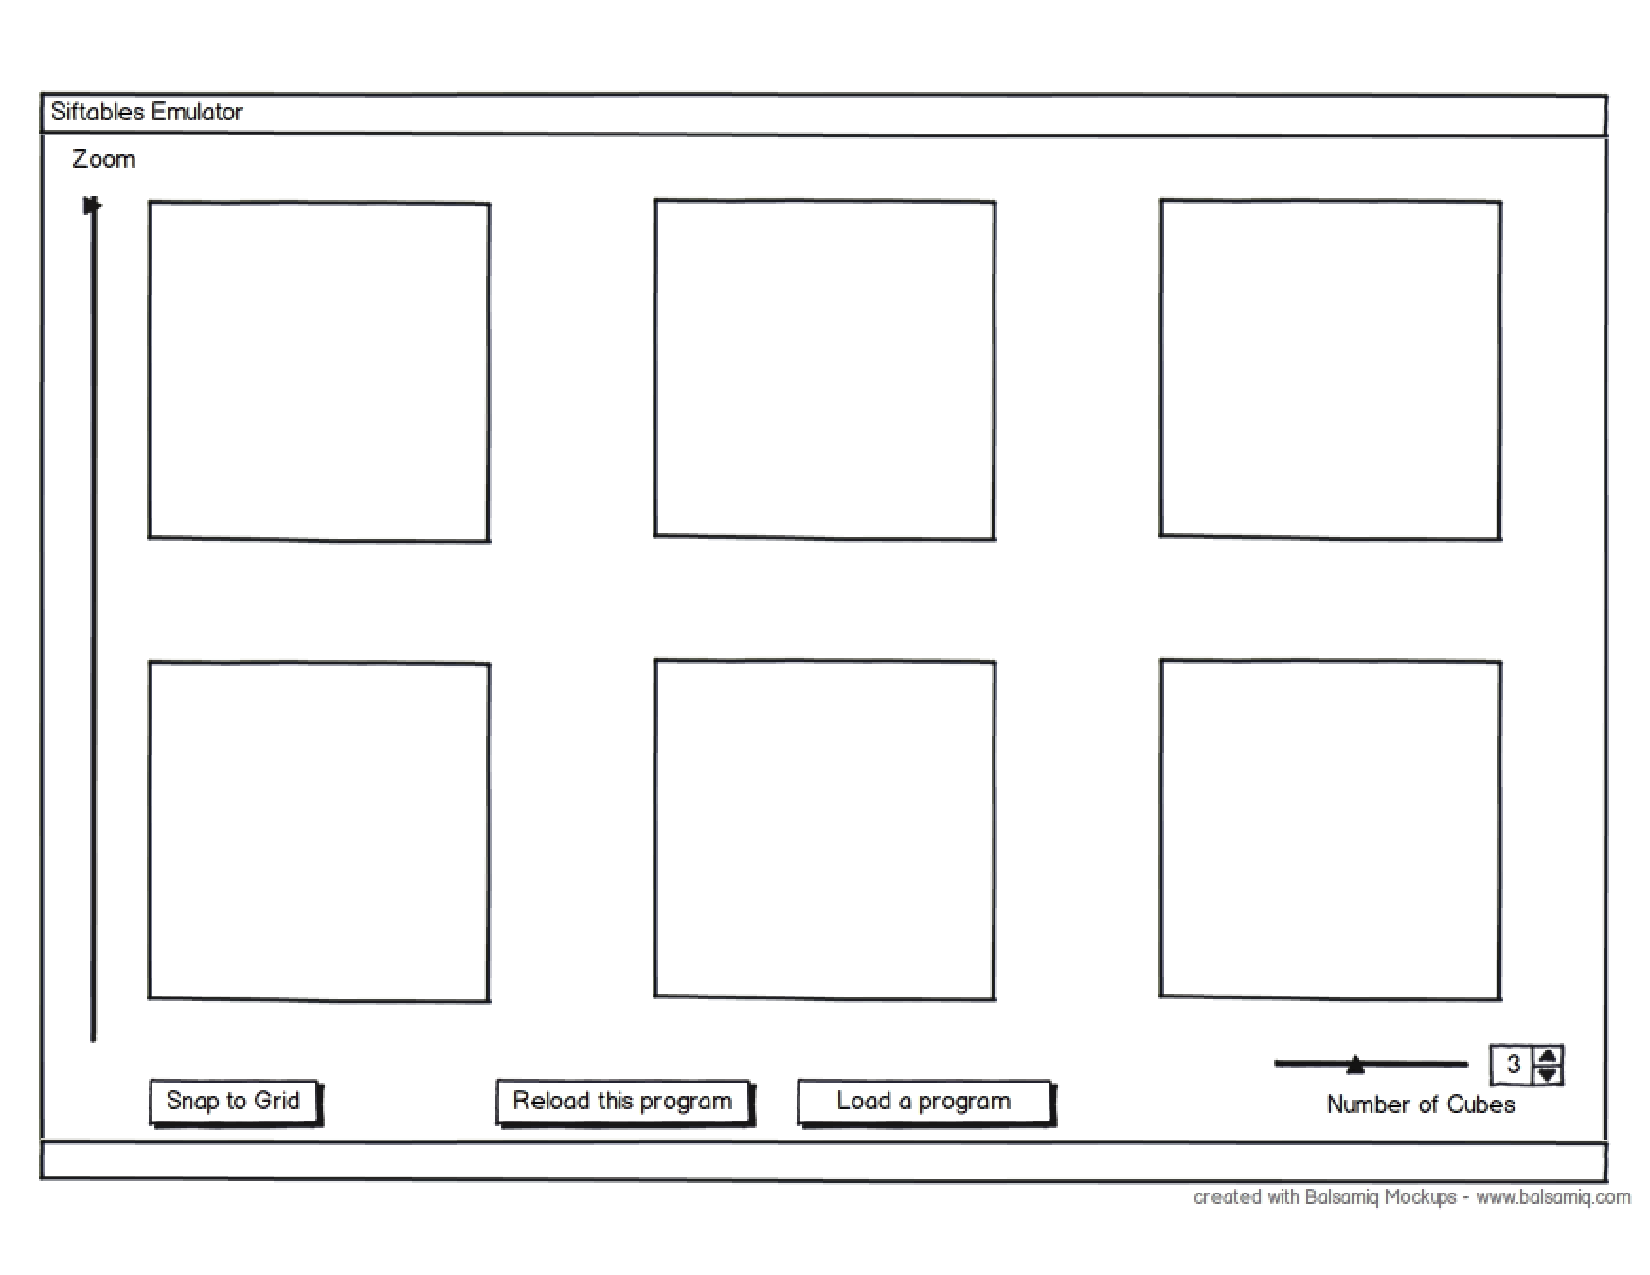
\includepdf[pages={1-3},landscape]{pdfs/mocks.pdf}

\appendix
    \begin{landscape}
    \section{Features}
    \begin{table}[h!]
      \begin{tabular}{p{.25in} | p{2.75in} | p{3in} | p{3in}}
        \textbf{ID} &
        \textbf{Feature} &
        \textbf{Description} &
        %\textbf{Status} &
        %\textbf{Priority} &
        %\textbf{Risk} &
        %\textbf{Stability} &
        \textbf{Reason} 
        %\textbf{Effort}
        \\ \hline

        F1 &
        Individual, virtual Sifteo Cube &
        A virtual representation of a single Sifteo Cube &
        %Approved &
        %Critical &
        %Low &
        %High &
        Replicates physical Sifteo Cube
        %Medium 
        \\ \hline

        F2 &
        Buttons to manipulate each virtual Cube &
        Buttons on the virtual Cube will allow the User to flip and tilt it &
        %Approved &
        %Critical &
        %Medium &
        %High &
        Replaces physical actions where said actions would be impractical with a mouse
        %Medium
        \\ \hline

        F3 &
        Workspace where multiple Cubes can be emulated &
        Multiple Cubes will be displayed on a workspace that replicates the free-form nature of physical Sifteo Cubes\index{Sifteo Cubes} &
        %Approved &
        %Critical &
        %Low &
        %High &
        Replicates multiple Sifteo Cubes\index{Sifteo Cubes} in a natural, free-form environment
        %High
        \\ \hline

        F4 &
        Interactions between Cubes &
        The Cubes present on the workspace will communicate when they are neighbored &
        %Approved &
        %Critical &
        %Low &
        %High &
        Cubes can simulate the interactions possible with physical Cubes
        %High 
        \\ \hline

        F5 &
        Load programs into the Cubes &
        The User will load his own and example programs into the emulator’s\index{emulator} Cubes &
        %Approved &
        %Critical &
        %Medium &
        %High &
        The ability to program programs for the emulator\index{emulator} is dependent on a common interface
        %High
        \\ \hline

        F6 &
        Snap Cubes to invisible grid &
        The Cubes will snap into an invisible grid when a button is clicked &
        %Proposed &
        %Useful &
        %Medium &
        %High &
        Increases productivity by allowing a quick reset if the Cubes are in disarray
        %Low
        \\ \hline

        F7 &
        Zoom Workspace &
        The Workspace will zoom to the level of an individual Cube or the whole space &
        %Proposed &
        %Useful &
        %Low &
        %High &
        Inspecting individual Cubes allows for precise checks of program \glspl{GUI}\index{GUI}\glsadd{GUIa}
        %Low
        \\ \hline

      \end{tabular}
    \end{table}
    \end{landscape}

\clearpage
\addcontentsline{toc}{section}{Glossary}
\printglossaries
\clearpage

\addcontentsline{toc}{section}{References}
\section*{References}

        \begin{enumerate}
                \item{Sifteo Inc. Online: http://www.sifteo.com}
                \item{Tim Ekl.  Client Meeting.  12 September 2011 12:45 p.m.}
        \end{enumerate}

\clearpage

\addcontentsline{toc}{section}{Index}
\printindex

\end{document}
